\documentclass[elementsmain.tex]{subfiles}
\begin{document}
\section{The Dot Product and Geometry}

A lot of the basic geometry of $\R^n$ is captured by a mysterious object called the \emph{dot product}. First, we will show how this can be understood in $\R^2$, and then we will generalize everything to $\R^n$ for $n\geq 2$.

\subsection*{Lengths and Angles in $\R^2$}

Given two vectors, their dot product is a real number. This number is a strange measure of how much the vectors are alike, and captures information about both lengths and angles. The formal definition is this.

\begin{definition}[The Dot Product in $\R^2$]
Let $u = \smvec{u_1}{u_2}$ and $v = \smvec{v_1}{v_2}$ be vectors in $\R^2$. 
The \emph{dot product} of $u$ and $v$ is the number
\[
u\cdot v = u_1v_1 + u_2v_2 .
\]
\end{definition}

The clearest geometric information we can pull out of the dot product is about lengths.

\begin{theorem}[Lengths in $\R^2$]
Let $u = \smvec{a}{b} \in \R^2$ be a vector. The length of $u$ is equal to the square root of the dot product of $u$ with itself. That is, the length of $u$ is
\[
\sqrt{u\cdot u\,} = \sqrt{a^2+b^2\,}
\]
\end{theorem}

\begin{proof}
The key comes from considering Figure \ref{fig:norm}. 
There we see the vector $u$ in $\R^2$ is the hypotenuse of a right triangle 
having its legs parallel to the two coordinate axes.

\begin{figure}[h!]
\centering
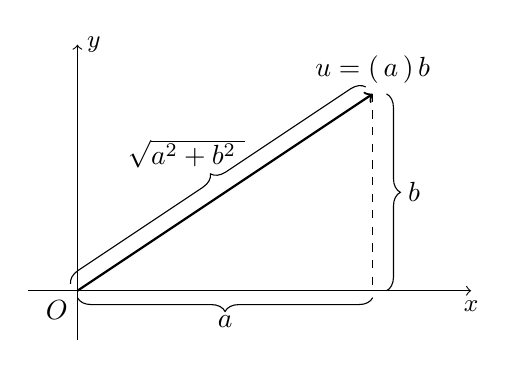
\begin{tikzpicture}[scale=1.25]
\draw[->] (-.5,0) -- (4,0) node[below] {\small $x$};
\draw[->] (0,-.5) -- (0,2.5) node[right] {\small $y$};
\node[below left] at (0,0) {$O$};
\draw[->,thick] (0,0) -- (3,2) node[above] {$u = \begin{pmatrix} a \\ b\end{pmatrix}$};
\draw[dashed] (3,2) -- (3,0);
\draw[decorate,decoration={brace,mirror,amplitude=5pt},xshift=4pt,yshift=0pt] (3,0) -- (3,2) node[midway,xshift=.35cm] {$b$};
\draw[decorate,decoration={brace,mirror,amplitude=5pt},xshift=0pt,yshift=-2pt] (0,0) -- (3,0) node[midway,yshift=-.3cm] {$a$};
\draw[decorate,decoration={brace,amplitude=5pt},xshift=-2pt,yshift=2pt] (0,0) -- (3,2) node[midway,xshift=-.4cm,yshift=.4cm] {$\sqrt{a^2+b^2\ }$};
\end{tikzpicture}
\caption{The Norm of a vector}
\label{fig:norm}
\end{figure}

These two legs then have lengths which are equal to our two coordinates, respectively.
So we can compute the length of the hypotenuse (our vector) by the Pythagorean Theorem, which completes our proof.
\end{proof}

The length of a vector is a useful concept, but mathematicians often use another name for it. New learners often find this confusing, so beware!

\begin{definition}[Norm, Unit Vector]
Let $u = \smvec{a}{b}$ be a vector in $\R^2$.
The \emph{norm} of $u$ is the number
\[
\norm{u} = \sqrt{u\cdot u\,} = \sqrt{a^2 + b^2\,}.
\]
We say that $u$ is a \emph{unit vector} when it has a norm of $\norm{u}=1$.
\end{definition}




\begin{theorem}[The Norm and Scalar Multiplication]
Let $\lambda$ be a scalar, and let $u\in \R^2$ be a vector. Then
\[
\norm{\lambda u}
= |\lambda| \norm{u}
\]

\end{theorem}

This conforms to our basic ideas about scalar multiplication. If we rescale a vector, we are really just changing its length by that factor. (And then there is the worry over the sign of the scalar, because lengths must not be negative.)


\begin{proof}
Suppose that the vector is $u =\smvec{a}{b} $.
We can do the following straightforward computation:
\[
\begin{split}
\norm{\lambda u} & = \norm{ \lambda \begin{pmatrix} a \\ b \end{pmatrix}} = \norm{ \begin{pmatrix} \lambda a \\ \lambda b \end{pmatrix} } = \sqrt{ (\lambda a)^2 + (\lambda b)^2\ } \\
& = \sqrt{\lambda^2(a^2+b^2)\,} = |\lambda| \sqrt{a^2+b^2\,}\\
& = |\lambda| \norm{u}
\end{split}
\]
Since the first and last are equal, we have established the desired result.
\end{proof}


In a terrible linguistic collision, the most useful role for the norm of a vector is in the process of \emph{normalizing} that vector. 
Beware! Mathematics has several words that are overused! 
Norm, normal, normalize, normalized and other forms of this are a prime example.
To \emph{normalize} a vector $u$, we multiply it by the scalar $\norm{u}^{-1}$, and thus produce a new vector $u/\norm{u}$ which points in the same direction as $u$, but has norm equal to $1$. This is because we can use our observation just above about how norms interact with scalar multiplication to compute:
\[
\norm{\norm{u}^{-1} u} = \norm{u}^{-1}\norm{u}  = 1.
\]
That last multiplication is just a multiplication of numbers.
Note that all of that only makes sense as long as $u$ is not the zero vector. If $u$ is the zero vector, its norm is $\norm{u}=0$. Since it makes no sense to divide by zero, it is not possible to normalize the zero vector.

To sum up: given a non-zero vector $u$, it is possible to normalize it, which means to replace it with the unit vector $u/\norm{u}$.\\


Let's turn out attention to measuring angles between vectors. To do this properly, we will need a little trigonometry. The three necessary facts are collected in the next theorem as a refresher. 

\begin{theorem}[Some Trigonometry]\label{thm:trig}
The following statements are true.
\begin{enumerate}
\item Each point on the unit circle can be represented as a point of the form $(\cos(\alpha), \sin(\alpha))$ for some angle $\alpha$ between $0$ and $2\pi$, so the corresponding vector can be written as $p = \smvec{\cos(\alpha)}{\sin(\alpha)}$.


\begin{figure}[h]
\centering
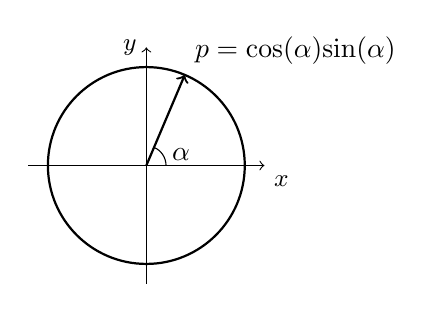
\begin{tikzpicture}[scale=1.25]
\draw[->] (-1.2,0) -- (1.2,0) node[below right] {\small $x$};
\draw[->] (0,-1.2) -- (0,1.2) node[left] {\small $y$};
\draw[thick] (0,0) circle [radius=1];
\draw[thick,->] (0,0) -- (67:1) node[above right] {$p = \smvec{\cos(\alpha)}{\sin(\alpha)}$};
\draw (.2,0) arc [radius=0.2,start angle=0,end angle=67];
\node[right] at (35:.2) {$\alpha$};
\end{tikzpicture}
\caption{Trigonometry for points on the unit circle}
\label{fig:unit-circle}
\end{figure}


\item The function $\theta \mapsto \cos(\theta)$ associates to each angle in the interval
$[0,\pi]$ a unique real number in the interval $[-1,1]$, and vice versa.  In particular, this function has a sensible inverse function $\arccos: [-1,1]\rightarrow [0,\pi]$. For us, this means that it to measure an angle, we can get away with instead finding the cosine of that angle.

\begin{figure}[h]
\centering
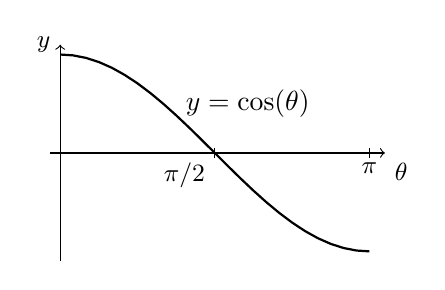
\begin{tikzpicture}[scale=1.25]
\draw[->] (-.1,0) -- (3.3,0) node[below right] {\small $\theta$};
\draw[->] (0,-1.1) -- (0,1.1) node[left] {\small $y$};
\draw [thick,domain=0:pi] plot (\x, {cos(\x r)});
\node[right] at (3*pi/8,1/2) {$y=\cos(\theta)$};
\draw[-] (pi/2,-.05) -- (pi/2,.05);
\draw[-] (pi,-.05) -- (pi,.05);
\node[below left] at (pi/2,0) {\small $\pi/2$};
\node[below] at (pi,0) {\small $\pi$};
\end{tikzpicture}
\caption{Part of the graph of $y=\cos(\theta)$}
\label{fig:cos-graph}
\end{figure}

\item There is an identity on trigonometric functions that helps us deal with the the cosine of a difference of angles: If $\alpha$ and $\beta$ are two angles, then
\[
\cos(\beta-\alpha) = \cos(\alpha)\cos(\beta) + \sin(\alpha)\sin(\beta).
\]
\end{enumerate}
\end{theorem}


You might recognize all of these facts from a trigonometry or pre-calculus class. In any case, you should take them as true. It would take us too far out of our studies to establish them now.


\begin{theorem}[Angles in $\R^2$]
Let $u, v \in \R^2$ be two vectors. Then the angle $\theta$ between $u$ and $v$ is 
\[
\theta = \arccos\left(\dfrac{u\cdot v}{\norm{u}\norm{v}}\right).
\]
\end{theorem}

\begin{proof}
So, we consider the angle between two vectors, $u$ and $v$, in $\R^2$. As they are mathematician's vectors, they are both based at the origin, and naturally form an angle there. We will now apply each of the facts from Theorem \ref{thm:trig}.

Note that the angle between these vectors does not depend at all on their lengths. 
If we change one, or both, of the vectors by rescaling them, that will not change the directions involved, and hence will not change the angle we seek. 
We can get to a more uniform set up for our task by normalizing $u$ and $v$. 
Thus, we will instead consider the unit vectors $u/\norm{u}$ and $v/\norm{v}$, and look for the angle $\theta$ between them as in Figure \ref{fig:angle-computation}.

Since our new vectors are unit vectors, we can represent them with trigonometric functions:
\[
\frac{u}{\norm{u}} = \begin{pmatrix} \cos(\alpha)\\ \sin(\alpha) \end{pmatrix}, \qquad
\frac{v}{\norm{v}} = \begin{pmatrix} \cos(\beta)\\ \sin(\beta) \end{pmatrix}.
\]
Let's suppose that the angle $\beta$ that $v$ makes with the $x$-axis is larger than the angle $\alpha$ that $u$ makes with the $x$-axis. Then we want to find the angle $\theta = \beta-\alpha$. 

\begin{figure}[h!]
\centering
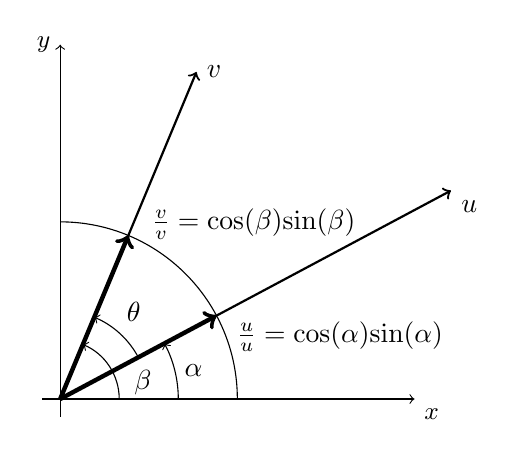
\begin{tikzpicture}[scale=2.25]
\draw[->] (-.1,0) -- (2,0) node[below right] {\small $x$};
\draw[->] (0,-.1) -- (0,2) node[left] {\small $y$};
\draw (1,0) arc [radius=1,start angle=0,end angle=90];
\draw[thick,->] (0,0) -- (10/13,24/13) node[right] {$v$};
\draw[ultra thick,->] (0,0) -- (5/13,12/13);
\node [above right] at (6/13,11/13) {$\frac{v}{\norm{v}}=\smvec{\cos(\beta)}{\sin(\beta)}$};
\draw[thick,->] (0,0) -- (37.5/17,20/17) node[below right] {$u$};
\draw[ultra thick,->] (0,0) -- (15/17,8/17);
\node [right] at (16/17,6/17) {$\frac{u}{\norm{u}}=\smvec{\cos(\alpha)}{\sin(\alpha)}$};
\draw[->] (2/3,0) arc [radius=2/3,start angle=0,end angle=28];
\node[right] at (14:2/3) {$\alpha$};
\draw[->] (1/3,0) arc [radius=1/3,start angle=0,end angle=67.38];
\node[right] at (14:3/8) {$\beta$};
\draw[->] (28:1/2) arc [radius=1/2,start angle=28,end angle=67.38];
\node[above right] at (50:1/2) {$\theta$};
\end{tikzpicture}
\caption{Finding the angle between two vectors.}
\label{fig:angle-computation}
\end{figure}

By angle difference formula for cosine, we have
\[
\begin{split}
\cos(\theta) & = \cos(\beta - \alpha) \\
& = \cos(\alpha)\cos(\beta) + \sin(\alpha)\sin(\beta)\\
& = \left( \frac{u}{\norm{u}}\right) \cdot \left( \frac{v}{\norm{v}} \right) \\
& = \dfrac{u\cdot v}{\norm{u}\norm{v}}.
\end{split}
\]
Now, we apply the function $\arccos$ to both sides to get the theorem.
\end{proof}


As our study progresses, we will not have much use for measuring particular angles, but it will be very important to us to understand situations when two vectors make an angle of $\pi/2$ radians (i.e. $90^{\circ}$, a right angle). It is common in geometry to call such vectors \emph{perpendicular}. It is a fact that $\cos(\pi/2) = 0$, so that non-zero vectors $u$ and $v$ make an angle of $\pi/2$ when
\[
0 = \cos(\pi/2) = \dfrac{u\cdot v}{\norm{u}\norm{v}}.
\]
By clearing out the denominator of this fraction, we see that $u$ and $v$ make an angle of $\pi/2$ exactly when $u\cdot v = 0$. In another instance of cluttering the vocabulary list for math students, in a linear algebra context such vectors are called by yet another term.

\begin{definition}[Orthogonal Vectors]
We say that two vectors $u$ and $v$ in $\R^2$ are \emph{orthogonal} when $u\cdot v = 0$.
\end{definition}


\subsection*{The Dot Product in $\R^n$}

Now we will give the general definition and results. Fortunately, everything works the same.

\begin{definition}[The Dot Product]
Let $u$ and $v$ be vectors in $\R^n$ with coordinates labeled like those below.
\[
u = \begin{pmatrix}u_1 \\ u_2 \\ \vdots \\ u_n\end{pmatrix}, \quad
v = \begin{pmatrix}v_1 \\ v_2 \\ \vdots \\ v_n\end{pmatrix} 
\] 
The \emph{dot product} of $u$ and $v$ is the number
\[
u\cdot v = u_1v_1 + u_2v_2 + \dots + u_nv_n.
\]
\end{definition}

Once we have the dot product available, we can work by analogy to define all of the other new words of this section for vectors in $\R^n$, too.

\begin{definition}[Geometry in $\R^n$]
Let $u, v \in \R^n$ be vectors. 
\begin{itemize}
\item The \emph{norm of $u$} is $\norm{u} = \sqrt{u\cdot u\ }$. 
\item The vector $u$ is called a \emph{unit vector} when $\norm{u}=1$.
\item The \emph{angle between $u$ and $v$} is the number 
\[
\theta = \arccos\left(\frac{u\cdot v}{\norm{u}\norm{v}}\right).
\]
\item We say that $u$ and $v$ are \emph{orthogonal} when $u\cdot v = 0$.
\end{itemize}
\end{definition}



The next two theorems are not hard to prove, but they are tedious. In each case,
one has to argue one coordinate at a time, using a relevant property for real numbers.
It is best to just check them for some examples until you understand and believe them.

\begin{theorem}[Algebra of the Dot Product]
Let $u$, $v$, and $w$ be vectors in $\R^n$ and let $\lambda$ and $\mu$ be scalars. Then
\begin{itemize}
\item The dot product is \emph{symmetric}: $u\cdot v = v \cdot u$;
\item The dot product \emph{distributes} over linear combinations 
\[
u \cdot (\lambda v + \mu w) = \lambda (u\cdot v) + \mu (u\cdot w)
\]
\end{itemize}
\end{theorem}


\begin{theorem}[Algebra of the Norm]
Let $u \in \R^n$ be a vector, and let $\lambda$ be a scalar. Then 
\begin{itemize}
\item $\norm{u} \geq 0$.
\item $\norm{u} = 0$ if, and only if, $u$ is the zero vector.
\item $\norm{\lambda u} = |\lambda| \norm{u}$
\end{itemize}
\end{theorem}


\clearpage

\subsection*{Exercises}

\begin{exercise}
Choose three different vectors in $\R^2$ which have neither of their components equal to zero. Call these vectors $u$, $v$, and $w$.
\begin{compactitem}
\item[a)] Compute the norms of $u$, $v$, and $w$.
\item[b)] Compute the dot products $u\cdot v$, $v\cdot w$, and $u\cdot w$.
\item[c)] Find unit vectors $u'$, $v'$, and $w'$ which point in the same directions as $u$, $v$, and $w$, respectively.
\item[d)] Find the angles between each of the pairs, $u$ and $v$, $u$ and $w$, $v$ and $w$ in radians.
\end{compactitem}
\end{exercise}



\begin{exercise}
Fix some vector $u \in\R^2$. Draw a picture of $u$ in the plane, and then shade the region of the plane which contains vectors $v$ so that $u\cdot v> 0$.
\end{exercise}



\begin{exercise} This task continues our quest for understanding the sign of a dot product geometrically.
\begin{compactitem}
\item[a)] Find an example of two $v$ and $w$ in $\R^2$ so that $\left(\begin{smallmatrix}1 \\ 2 \end{smallmatrix}\right)\cdot v =0$ and $\left(\begin{smallmatrix}1 \\ 2 \end{smallmatrix}\right)\cdot w = 0$, or explain why such an example is not possible.

\item[b)] Let $v = \left(\begin{smallmatrix}3\\-1 \end{smallmatrix}\right)$. Find an example of a pair of $2$-vectors $u$ and $w$ such that $v \cdot u < 0$ and $v \cdot w < 0$ and $w \cdot u = 0$, or explain why no such pair of vectors can exist.

\item[c)] Find an example of three $2$-vectors $u$, $v$, and $w$ so that $u \cdot v < 0$ and $u\cdot w < 0$ and $v \cdot w < 0$, or explain why no such example exists.
\end{compactitem}
\end{exercise}

\begin{exercise}
What shape is the set of solutions $\left(\begin{smallmatrix} x \\ y \end{smallmatrix}\right)$ to the equation
\[
\begin{pmatrix} 3 \\ 7\end{pmatrix} \cdot \begin{pmatrix} x \\ y \end{pmatrix} = 5?
\] 
That is, if we look at all possible vectors $\left(\begin{smallmatrix} x \\ y \end{smallmatrix}\right)$
which make the equation true, what shape does this make in the plane? Draw this shape.

What happens if we change the vector $\left(\begin{smallmatrix} 3 \\ 7 \end{smallmatrix}\right)$ to some other vector? What happens if we change the number $5$ to some other number?
\end{exercise}


\begin{exercise}
\begin{compactitem}
\item[a)] Find an example of a number $c$ so that the equation
\[
\begin{pmatrix} 1 \\ -1 \end{pmatrix} \cdot \begin{pmatrix} x \\ y \end{pmatrix} = c
\]
has the vector $\left(\begin{smallmatrix}4 \\ 7 \end{smallmatrix}\right)$ as a solution, or explain why no such number exists.
\item[b)] Let $v = \left(\begin{smallmatrix}2\\1\end{smallmatrix}\right)$ and $w=\left(\begin{smallmatrix}-3\\4\end{smallmatrix}\right)$. Find an example of a number $c$ so that 
\begin{gather*} 
v \cdot \begin{pmatrix}1\\-1\end{pmatrix} = c \quad\text{ and } \quad w \cdot \begin{pmatrix}1\\-1\end{pmatrix} = c, 
\end{gather*}
or explain why this is not possible.
\item[c)] Let $P = \left(\begin{smallmatrix}-3\\4\end{smallmatrix}\right)$. Find an example of numbers $c$ and $d$ so that 
\begin{gather*} \begin{pmatrix} 2\\-1\end{pmatrix}\cdot P = c \quad\text{ and } \quad \begin{pmatrix} 1\\-1\end{pmatrix}\cdot P = d, 
\end{gather*} 
or explain why no such example is possible.
\end{compactitem}
\end{exercise}

\begin{exercise}
Write down two vectors in $\R^3$ which have no coordinates equal to zero. Call them $u$ and $v$. Find the following things:
\begin{compactitem}
\item The dot product $u\cdot v$;
\item The norms of $u$ and $v$;
\item unit vectors which point in the same directions as $u$ and $v$, respectively; and
\item the angle between $u$ and $v$.
\end{compactitem}
\end{exercise}



\end{document}